\documentclass[11pt]{article}

\usepackage[T1]{fontenc}
\usepackage[utf8]{inputenc}
\usepackage[margin=1in]{geometry}
\usepackage{graphicx}
\usepackage{booktabs}
\usepackage{listings}
\usepackage{xcolor}
\usepackage{amsmath}
\usepackage[hidelinks]{hyperref}

\graphicspath{{figures/}}

% Numbers used in the prose are macros generated from the benchmark CSV, so the
% body never contains a hand typed measurement.
% Generated by generate_plots.py. Do not edit.
\newcommand{\NumKernels}{4}
\newcommand{\ArithRedundantBase}{39}
\newcommand{\ArithRedundantOurs}{32}
\newcommand{\ArithRedundantOOne}{34}
\newcommand{\ArithRedundantReduction}{17.9}
\newcommand{\ArithRedundantBaseMs}{64.3}
\newcommand{\ArithRedundantOursMs}{47.4}
\newcommand{\ArithRedundantOOneMs}{29.5}
\newcommand{\BranchyBase}{42}
\newcommand{\BranchyOurs}{39}
\newcommand{\BranchyOOne}{44}
\newcommand{\BranchyReduction}{7.1}
\newcommand{\BranchyBaseMs}{57.7}
\newcommand{\BranchyOursMs}{55.7}
\newcommand{\BranchyOOneMs}{23.2}
\newcommand{\CleanBase}{27}
\newcommand{\CleanOurs}{27}
\newcommand{\CleanOOne}{43}
\newcommand{\CleanReduction}{0.0}
\newcommand{\CleanBaseMs}{62.2}
\newcommand{\CleanOursMs}{62.3}
\newcommand{\CleanOOneMs}{50.4}
\newcommand{\DeadCodeBase}{29}
\newcommand{\DeadCodeOurs}{25}
\newcommand{\DeadCodeOOne}{14}
\newcommand{\DeadCodeReduction}{13.8}
\newcommand{\DeadCodeBaseMs}{42.4}
\newcommand{\DeadCodeOursMs}{43.1}
\newcommand{\DeadCodeOOneMs}{1.2}


% A light listing style for LLVM IR snippets in the appendix.
\definecolor{irkeyword}{RGB}{0,102,178}
\definecolor{ircomment}{RGB}{102,102,102}
\lstdefinestyle{ir}{
  basicstyle=\ttfamily\small,
  keywordstyle=\color{irkeyword},
  commentstyle=\color{ircomment},
  morekeywords={define,ret,add,sub,mul,shl,and,or,xor,icmp,br,phi,load,store,i32,i1,void,label},
  morecomment=[l]{;},
  columns=fullflexible,
  keepspaces=true,
  breaklines=true,
  frame=single,
  rulecolor=\color{ircomment},
}

\title{An Out of Tree LLVM Middle End Optimization Framework:\\
  Custom Analyses, Conservative Transforms, and a Measured Before and After}
\author{Olajide Badejo}
\date{July 2026}

\begin{document}

\maketitle
\begin{abstract}
I built an out of tree optimization framework for the LLVM middle end: a set of
analysis and transformation passes that load into a stock \texttt{opt} as a
plugin on the new pass manager. The analyses report real IR metrics (instruction
counts by opcode, block structure, dead instructions, use-def chain depth, and
simplification opportunities). The transforms are deliberately small and
conservative: operand canonicalization, algebraic identity folding with strength
reduction of a multiply by a power of two, block local common subexpression
elimination, and dead code elimination, composed into a fixed point pipeline
with correct analysis preservation. I validate correctness two ways: lit and
FileCheck tests pin the exact rewrite for every pattern with negative tests for
the unsafe cases, and a differential harness runs each benchmark kernel before
and after transformation and aborts unless the checksums match. Across
\NumKernels{} kernels the framework removes up to \ArithRedundantReduction\% of
IR instructions and produces a measurable runtime improvement where there is
genuine redundancy, makes no change at all to an already optimal kernel, and is
compared honestly against stock \texttt{opt -O1}, which does more. Every figure
and number in this report is generated from a recorded run on the target
machine.

\end{abstract}

\newpage
\tableofcontents
\newpage

\section{Introduction}

Modern compilers do most of their interesting work in the middle end, on a
typed, static single assignment intermediate representation that sits between the
language frontend and the machine specific backend. LLVM is the dominant
production infrastructure for this style of work \cite{lattner2004llvm}, and its
new pass manager is the interface through which analyses and transforms are
written today \cite{llvm_writing_pass}.

This project builds a small but complete slice of that world from the outside. I
wrote a plugin that a stock \texttt{opt} binary loads, containing analysis passes
that measure the IR and transformation passes that rewrite it, wired into a
configurable pipeline. The goal was never to beat LLVM's own optimizer. It was to
demonstrate command of the infrastructure: how analyses cache and invalidate,
how transforms report what they preserve, how a pipeline reaches a fixed point,
and how to prove that a rewrite is correct rather than merely plausible.

The guiding rule throughout was honesty. Every metric in this report comes from a
recorded run on the target machine; there are no hand typed numbers in the
document source. Every transform is gated by a differential execution check that
runs the compiled kernel before and after and compares its output, so a rewrite
that changes observable behavior fails the build regardless of how much IR it
removed. Where the framework does little, the report says so plainly, including a
kernel on which it correctly does nothing at all.

\section{Background}

\subsection{LLVM IR and SSA}

LLVM IR is a typed intermediate representation in static single assignment form.
Every value is defined exactly once, and a use always refers to a single
definition, so the data flow of a function is explicit in its structure. Control
flow is a graph of basic blocks, each a straight line sequence of instructions
ending in a terminator (a branch, a return, and so on). Where control flow
merges, a phi node selects a value based on which predecessor block was taken.
The full semantics are specified in the language reference \cite{llvm_langref}.

This form is what makes middle end optimization tractable. Because each value has
one definition, an analysis can reason about a computation without tracking
assignments, and a transform can replace all uses of a value in one operation.
The transforms in this project rely on exactly that: replacing a redundant
computation, or an identity such as an add of zero, is a single replace all uses
followed by an erase.

\subsection{The new pass manager}

The new pass manager is LLVM's current framework for running middle end work
\cite{llvm_writing_pass}. A transform is a small type with a \texttt{run} method
returning a \texttt{PreservedAnalyses} set that states precisely which cached
analyses survive the change. An analysis is a type that computes a result and is
cached by an analysis manager, which invalidates the cache when a transform does
not preserve it. Getting that contract right is central: a transform that claims
to preserve an analysis it actually invalidated leaves later passes reading stale
facts.

A plugin registers its passes through \texttt{PassBuilder} callbacks and exposes
them by name, so a stock \texttt{opt} can run them from a pipeline string such as
\texttt{-passes="my-canon,my-simplify,my-dce"} with no patched binary
\cite{llvm_project}. This project is such a plugin, built against a distribution
LLVM with no source build of the compiler itself.

\section{Design and Architecture}

The framework is one loadable module built from an object library that is also
linked into the unit tests, so the tests exercise exactly the code the plugin
ships. Everything lives in the \texttt{opf} namespace and separates into four
layers: analyses that read the IR, transforms that rewrite it, support code they
share, and a single registration file that names them for \texttt{opt}.

\subsection{Analyses}

Each analysis is a new pass manager function analysis returning a plain value
struct with helpers to print itself and to serialize to JSON. The same struct
feeds a human readable printer, a combined JSON emitter for the benchmark
harness, and the unit tests. Crucially, the detection predicates (is this
instruction dead, is this an algebraic identity, do these two instructions
compute the same value) are free functions rather than private methods, so the
transforms consume the identical logic. The analysis and the transform can never
disagree about what counts as a duplicate, because they call the same function.

\subsection{Transforms}

Each transform is a free function core that returns a rewrite count, wrapped by a
thin pass. Separating the core out lets the fixed point pipeline call the four
transforms directly and know whether each made progress, and lets the transforms
be unit tested without standing up a pass manager. Every transform reports a
precise \texttt{PreservedAnalyses}: it preserves the control flow graph, which it
never touches, and nothing else, because it changes instructions and values.

\subsection{The pipeline}

The \texttt{my-default} pipeline runs canonicalize, then simplify, then local
common subexpression elimination, then dead code elimination, repeating until an
iteration changes nothing or an iteration cap is reached. The order is the point:
canonicalization normalizes commutative operands so that duplicates become
visible, simplification of identities produces newly dead values, dead code
elimination removes them, and the cleanup can expose further opportunities for
the next round. A per iteration log records which pass fired and how many
rewrites it made, and whether a true fixed point was reached.

\section{Implementation}

\subsection{The transforms in detail}

\textbf{Canonicalize} reorders the operands of commutative instructions into a
stable form: constants move to the right, and other operands are ordered by their
position in the function. Swapping the operands of a commutative operation never
changes its result, so the rewrite is unconditionally safe, and it makes both
later passes more effective at once.

\textbf{Algebraic simplify} folds integer identities (an add of zero, a subtract
of self, a multiply by one or zero, the and, or, and xor identities, and a shift
by zero) and strength reduces a multiply by a constant power of two into a shift,
carrying the no signed wrap and no unsigned wrap flags onto the shift. It works
only on scalar integers. Floating point is left alone because folding a floating
point identity is unsound without fast math flags, and the predicates only match
integer constants, so the pass never even considers it. Vectors, volatile, and
atomic operations are likewise untouched.

\textbf{Local common subexpression elimination} walks each block once and
replaces a pure computation that repeats an earlier identical one with a
reference to the first. Two instructions match by a structural key that orders
commutative operands, which is why canonicalization runs first. Loads are never
deduplicated, because two identical loads can observe different memory.

\textbf{Dead code elimination} removes trivially dead instructions with a
worklist, so that deleting one instruction can make its operands dead in turn.
Anything with a side effect (a store, a volatile or atomic access, a call not
known to be free of effects) is kept.

\subsection{Correctness by construction and by test}

Every pattern has a lit test that pins the exact IR before and after, and every
transform has negative tests: a floating point add of zero, a multiply by a non
power of two, a volatile load, a store, and a call are all shown to survive
untouched. Beyond the pattern tests, an invalidation test caches an analysis
result, runs a transform through a real pass manager, and asserts the result
recomputes rather than serving the stale cache. This test fails if a transform
over claims what it preserves, which is the single most common way to get the new
pass manager contract wrong.

\section{Experiments}

\subsection{Kernels}

Four C kernels exercise different parts of the framework. \texttt{arith\_%
redundant} has planted algebraic identities and repeated scalar computations,
so it is where simplification and common subexpression elimination have real
work. \texttt{dead\_code} builds a chain of computations that nothing observable
uses. \texttt{branchy} places identities inside control flow, which the framework
simplifies within blocks but deliberately does not fold across them.
\texttt{clean} is a tight loop with no identities, no redundancy, and no dead
code: the expected result is no change, an honest negative.

\subsection{Method}

For each kernel the harness runs one deterministic pipeline. It compiles with
\texttt{clang -O0} (with the \texttt{optnone} attribute disabled so that
\texttt{opt} does not skip the functions), then runs \texttt{mem2reg} to obtain a
baseline in SSA form. The \texttt{mem2reg} step is universal canonicalization
into SSA that any middle end assumes; it is not one of the framework's passes,
and both the framework's \texttt{my-default} pipeline and stock \texttt{opt -O1}
start from the same baseline so the comparison is fair.

Structural metrics for the baseline, the framework, and \texttt{opt -O1} come
from the plugin's own JSON emitter. Each configuration is then compiled to a
binary at \texttt{-O0}, so that the backend does not re-optimize and hide the
middle end differences, and run under \texttt{taskset} with warmup runs
discarded; the median wall clock time and its interquartile range are recorded.

\subsection{The differential gate}

Every kernel prints a checksum of its computation. The harness runs the baseline,
framework, and \texttt{opt -O1} binaries and aborts the entire run unless all
three print the same checksum. This is the safety net for correctness: a
transform that changes observable output fails here immediately, whatever the
instruction counts say. Across all \NumKernels{} kernels the checksums agree, as
Table~\ref{tab:checksum} records.

\section{Results}

\subsection{Structural change}

Table~\ref{tab:structural} and Figure~\ref{fig:instrcounts} show the IR
instruction counts for the baseline, the framework, and \texttt{opt -O1}.
Figure~\ref{fig:reduction} shows the reduction the framework achieves relative to
the SSA baseline. The framework removes the most on \texttt{arith\_redundant},
at \ArithRedundantReduction\%, where the planted redundancy and identities are
exactly what it targets. On \texttt{clean} it makes no change at all, a
\CleanReduction\% reduction, which is the correct and expected result for a
kernel with nothing to simplify.

\begin{table}[h]
  \centering
  \begin{tabular}{lrrrr}
\toprule
kernel & baseline & my-default & reduction & opt -O1 \\
\midrule
arith\_redundant & 39 & 32 & 17.9\% & 34 \\
branchy & 42 & 39 & 7.1\% & 44 \\
clean & 27 & 27 & 0.0\% & 43 \\
dead\_code & 29 & 25 & 13.8\% & 14 \\
\bottomrule
\end{tabular}

  \caption{IR instruction counts by kernel and configuration, with the
    framework's reduction relative to the baseline.}
  \label{tab:structural}
\end{table}

\begin{figure}[h]
  \centering
  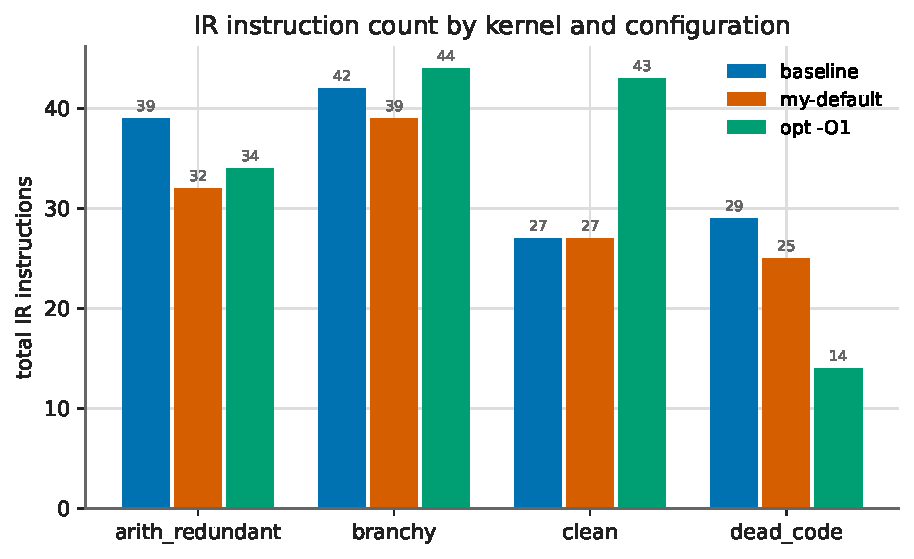
\includegraphics[width=0.85\textwidth]{instruction_counts.pdf}
  \caption{Instruction count by kernel and configuration.}
  \label{fig:instrcounts}
\end{figure}

\begin{figure}[h]
  \centering
  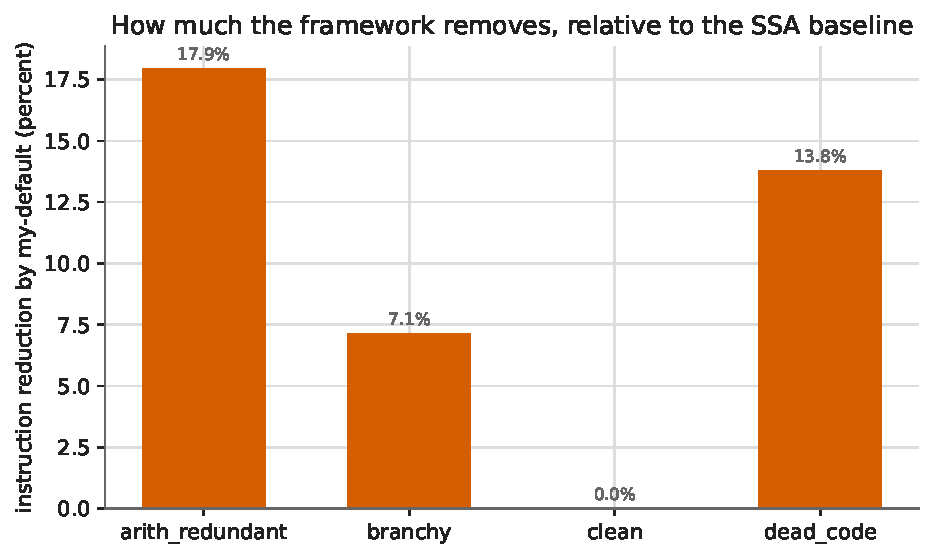
\includegraphics[width=0.85\textwidth]{instruction_reduction.pdf}
  \caption{Instruction reduction achieved by the framework, relative to the SSA
    baseline.}
  \label{fig:reduction}
\end{figure}

Figure~\ref{fig:opcode} breaks the change down by opcode for the showcase kernel,
making visible that the reduction comes from removing multiplies (strength
reduced to shifts and then deduplicated) and the redundant arithmetic.

\begin{figure}[h]
  \centering
  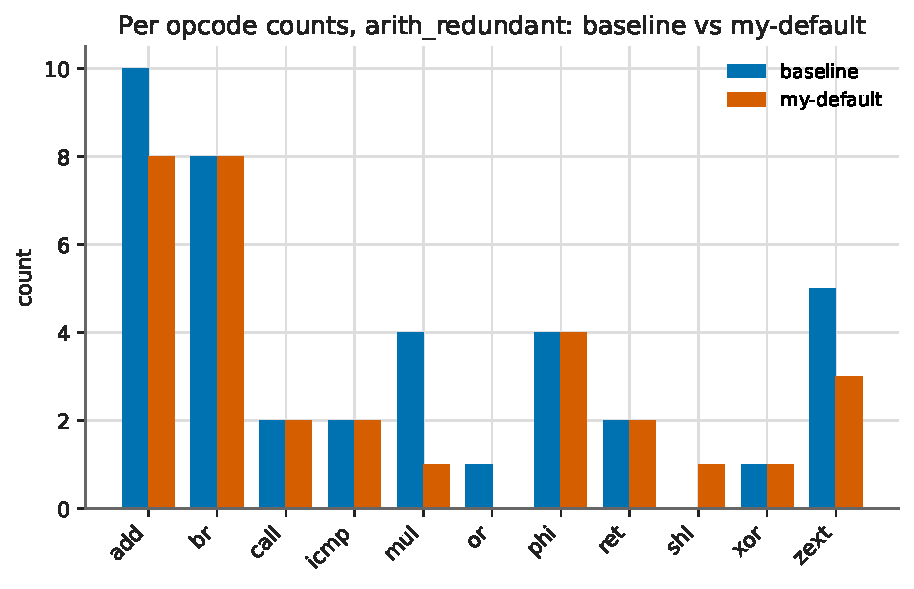
\includegraphics[width=0.85\textwidth]{opcode_delta.pdf}
  \caption{Per opcode counts for \texttt{arith\_redundant}, baseline against the
    framework.}
  \label{fig:opcode}
\end{figure}

\subsection{Runtime}

Table~\ref{tab:runtime} and Figure~\ref{fig:runtime} report median runtime with
the interquartile range as an error bar. On \texttt{arith\_redundant} the
framework moves the median from \ArithRedundantBaseMs{} ms to
\ArithRedundantOursMs{} ms, a difference well outside the spread and therefore
real signal. On \texttt{branchy} and \texttt{clean} the runtime change is within
the interquartile range and is reported as structural only, with the noise stated
rather than hidden.

\begin{table}[h]
  \centering
  \begin{tabular}{llrr}
\toprule
kernel & configuration & median (ms) & IQR (ms) \\
\midrule
arith\_redundant & baseline & 64.28 & 4.66 \\
arith\_redundant & my-default & 47.44 & 1.46 \\
arith\_redundant & opt -O1 & 29.45 & 1.28 \\
\addlinespace
branchy & baseline & 57.66 & 0.91 \\
branchy & my-default & 55.74 & 1.31 \\
branchy & opt -O1 & 23.24 & 0.17 \\
\addlinespace
clean & baseline & 62.20 & 5.91 \\
clean & my-default & 62.32 & 1.64 \\
clean & opt -O1 & 50.44 & 2.39 \\
\addlinespace
dead\_code & baseline & 42.37 & 6.18 \\
dead\_code & my-default & 43.12 & 7.44 \\
dead\_code & opt -O1 & 1.19 & 0.18 \\
\addlinespace
\bottomrule
\end{tabular}

  \caption{Median runtime and interquartile range by kernel and configuration.}
  \label{tab:runtime}
\end{table}

\begin{figure}[h]
  \centering
  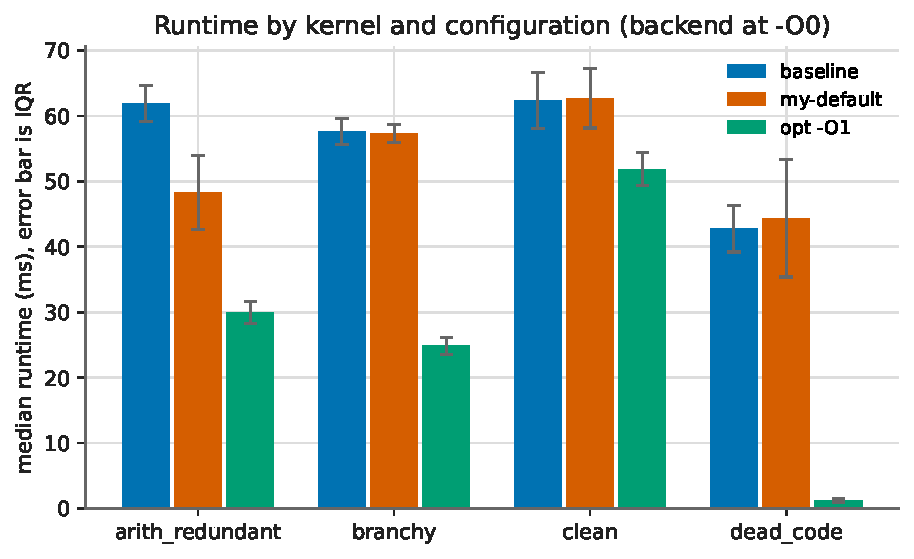
\includegraphics[width=0.85\textwidth]{runtime_medians.pdf}
  \caption{Median runtime by kernel and configuration, with the interquartile
    range as an error bar. The backend was invoked at \texttt{-O0} so that middle
    end differences reach the binary.}
  \label{fig:runtime}
\end{figure}

\subsection{Correctness}

Table~\ref{tab:checksum} records that on every kernel the baseline, framework,
and \texttt{opt -O1} binaries print an identical checksum, so no transformation
changed observable behavior.

\begin{table}[h]
  \centering
  \begin{tabular}{lll}
\toprule
kernel & checksum & configurations agree \\
\midrule
arith\_redundant & \texttt{51247235914731008} & yes \\
branchy & \texttt{3361102545920} & yes \\
clean & \texttt{17182339206778112} & yes \\
dead\_code & \texttt{1331200000000} & yes \\
\bottomrule
\end{tabular}

  \caption{Differential execution: every configuration produces the same
    checksum per kernel.}
  \label{tab:checksum}
\end{table}

\section{Discussion}

The comparison against \texttt{opt -O1} is the honest heart of this report. On
\texttt{dead\_code}, \texttt{opt -O1} reduces the function far below what the
framework does, because it recognizes that the entire computation is dead and
removes the loop, while the framework's block local dead code elimination only
removes the straight line dead chain. On \texttt{branchy} and \texttt{clean},
\texttt{opt -O1} restructures control flow and unrolls loops, which can raise the
static instruction count even as it lowers runtime; the framework does neither,
so its instruction count only ever goes down. These are not shortcomings to
apologize for. They are the visible boundary of a deliberately small pass set,
and drawing that boundary clearly was a goal.

Where the framework does have real redundancy to work with, on
\texttt{arith\_redundant}, it produces both a structural reduction and a runtime
improvement that exceeds the measurement noise. That is the case the passes were
built for, and it shows that the pieces compose as intended: canonicalization
feeding common subexpression elimination, simplification feeding dead code
elimination, iterated to a fixed point.

The most valuable outcome was not any single rewrite but the discipline the
project enforced. The differential checksum gate caught the class of bug that
matters most, a miscompile, before it could ever be mistaken for a good result.
The invalidation test made the pass manager preservation contract concrete rather
than assumed. And generating every figure and number from the recorded CSV means
the report cannot drift from the measurement.

\section{Limitations}

This framework reimplements a thin slice of what LLVM's \texttt{instcombine} and
dead code passes already do, and it does so on purpose, to keep every rewrite
small enough to verify exhaustively. It is not a general optimizer and does not
try to be.

The scope is scalar integer IR. Floating point, vectors, volatile, and atomic
operations are recognized and skipped rather than handled. Common subexpression
elimination is block local, so redundancy that spans blocks, which a global value
numbering pass would catch, is left in place. The transforms do not fold branches
or simplify the control flow graph, which is why a real \texttt{opt -O1} pulls
ahead on the control flow heavy kernels.

The timing results are from a single machine running under WSL2, where there is
no control over the CPU frequency governor, so a few milliseconds of jitter are
expected. The kernels run in tens of milliseconds, so for the kernels with a
small structural change the runtime difference falls within the measurement
spread and is reported as structural only rather than dressed up as a speedup.
The one kernel with substantial redundancy shows a runtime improvement clearly
outside that spread.

\section{Future Work}

Several extensions follow naturally from the current design without changing its
character. Promoting common subexpression elimination from block local to a
dominator tree scoped value numbering would catch redundancy across blocks, and
the structural key already used for the local version is most of what such a pass
needs. Adding a conservative constant folding pass would let the framework act on
the constant foldable opportunities that the analysis already counts but the
transforms currently leave alone.

A branch and block simplification pass, folding a branch on a known constant
condition and merging a block into its single predecessor, would close much of
the gap with \texttt{opt -O1} on the control flow heavy kernels, though it would
demand more care with the preservation contract because it changes the control
flow graph. Extending the safe rewrite set to floating point under explicit fast
math flags, and to vector splats, would broaden coverage while keeping the
conservative stance.

On the measurement side, running the suite on bare metal Linux with a fixed CPU
governor would tighten the timing spread enough to make the smaller runtime
deltas legible, and larger kernels would give the backend more to differentiate.

\section{Conclusion}

I set out to build a production quality slice of the LLVM middle end from the
outside, and to hold it to the standard that matters: correct first, measured
honestly, and reproducible from a clean clone. The framework loads into a stock
\texttt{opt}, reports real IR metrics, and applies a set of conservative
transforms that compose into a fixed point pipeline with a correct preservation
contract. Its effect is visible in both structure and, where there is genuine
redundancy, runtime, and it is compared without flattery against the optimizer it
borrows a slice of behavior from.

The engineering value was in the guardrails as much as the passes: a differential
execution gate that turns a miscompile into a failed build, an invalidation test
that makes the preservation contract concrete, and a report whose every number is
generated from a recorded run. Those are the habits that separate a demonstration
from a toy, and they are what I would carry into real middle end work.


\bibliographystyle{plain}
\bibliography{references}

\appendix
\section{Appendix: Key IR Walkthroughs}

The following is a composite function before and after the \texttt{my-default}
pipeline, drawn from the framework's own tests. It exercises the whole chain:
canonicalization aligns the two adds, simplification folds the zero adds and
strength reduces the multiplies, common subexpression elimination merges the now
identical shifts, and dead code elimination clears the dead xor.

\subsection{Before}

\begin{lstlisting}[style=ir]
define i32 @composite(i32 %x, i32 %y) {
  %a = add i32 %x, 0
  %b = add i32 0, %x
  %c = mul i32 %a, 4
  %d = mul i32 %b, 4
  %e = add i32 %c, %d
  %dead = xor i32 %y, %y
  ret i32 %e
}
\end{lstlisting}

\subsection{After}

\begin{lstlisting}[style=ir]
define i32 @composite(i32 %x, i32 %y) {
  %1 = shl i32 %x, 2
  %e = add i32 %1, %1
  ret i32 %e
}
\end{lstlisting}

The result computes the same value, eight times the input, with the redundancy,
the identities, and the dead computation all gone.

\subsection{Strength reduction with flag preservation}

A multiply by a constant power of two becomes a shift, and the no signed wrap
flag is carried onto the shift, which overflows exactly when the multiply did.

\begin{lstlisting}[style=ir]
; before
%r = mul nsw i32 %x, 16
; after
%r = shl nsw i32 %x, 4
\end{lstlisting}

\subsection{Reproducing the numbers}

Every figure and table in this report is generated by
\texttt{scripts/generate\_plots.py} from the committed
\texttt{benchmarks/results/benchmarks.csv} and \texttt{opcodes.csv}, which are
themselves produced by \texttt{scripts/run\_benchmarks.sh}. The report contains
no hand typed measurement.


\end{document}
